\documentclass{standalone}
\usepackage{tikz}
\usetikzlibrary{patterns, positioning}
\usepackage[sfdefault]{ClearSans} %% option 'sfdefault' activates Clear Sans as the default text font
\usepackage[T1]{fontenc}

\begin{document}
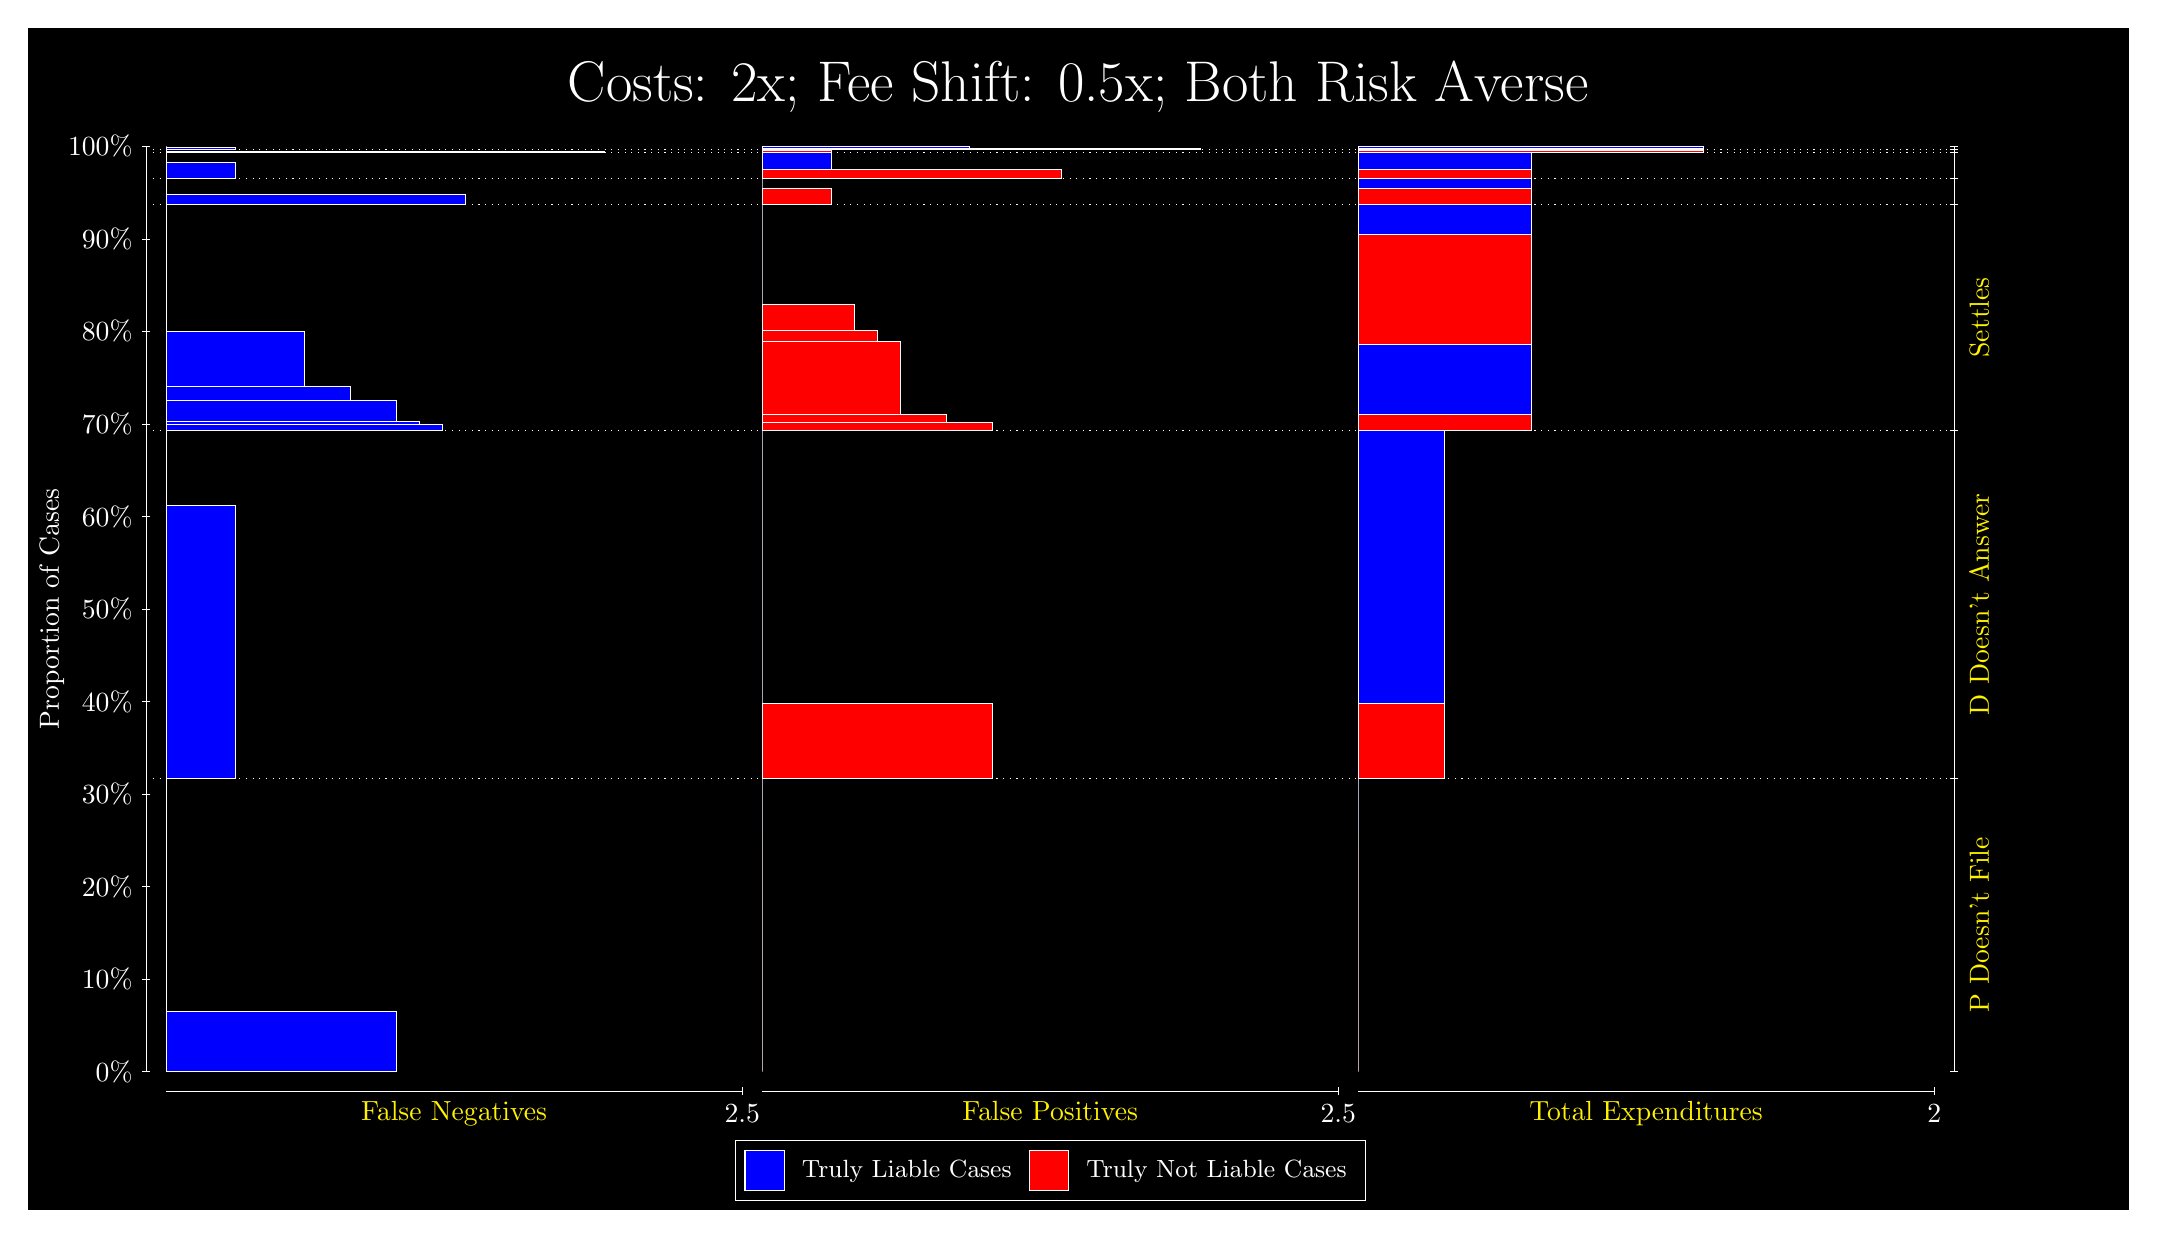
\begin{tikzpicture}
\draw[fill=black] (0,0) rectangle (26.667,15);
\draw[text=white] (0,13.5) rectangle (26.667,15) node[midway] {\huge Costs: 2x; Fee Shift: 0.5x; Both Risk Averse};
\draw[white, very thin] (1.5,1.75) -- (1.5,13.5);
\node[rotate=90, text=white, anchor=center] at (0.3, 7.625) {Proportion of Cases};
\draw[white, very thin] (1.45,1.75) -- (1.55,1.75);
\node[text=white, anchor=east] at (1.45, 1.75) {0\%};
\draw[white, very thin] (1.45,2.925) -- (1.55,2.925);
\node[text=white, anchor=east] at (1.45, 2.925) {10\%};
\draw[white, very thin] (1.45,4.1) -- (1.55,4.1);
\node[text=white, anchor=east] at (1.45, 4.1) {20\%};
\draw[white, very thin] (1.45,5.275) -- (1.55,5.275);
\node[text=white, anchor=east] at (1.45, 5.275) {30\%};
\draw[white, very thin] (1.45,6.45) -- (1.55,6.45);
\node[text=white, anchor=east] at (1.45, 6.45) {40\%};
\draw[white, very thin] (1.45,7.625) -- (1.55,7.625);
\node[text=white, anchor=east] at (1.45, 7.625) {50\%};
\draw[white, very thin] (1.45,8.8) -- (1.55,8.8);
\node[text=white, anchor=east] at (1.45, 8.8) {60\%};
\draw[white, very thin] (1.45,9.975) -- (1.55,9.975);
\node[text=white, anchor=east] at (1.45, 9.975) {70\%};
\draw[white, very thin] (1.45,11.15) -- (1.55,11.15);
\node[text=white, anchor=east] at (1.45, 11.15) {80\%};
\draw[white, very thin] (1.45,12.325) -- (1.55,12.325);
\node[text=white, anchor=east] at (1.45, 12.325) {90\%};
\draw[white, very thin] (1.45,13.5) -- (1.55,13.5);
\node[text=white, anchor=east] at (1.45, 13.5) {100\%};

\draw[white, very thin] (24.457,1.75) -- (24.457,13.5);
\draw[white, very thin] (24.407,1.75) -- (24.507,1.75);
\node[anchor=west] at (24.407, 1.75) {};
\draw[white, very thin] (24.407,5.4737) -- (24.507,5.4737);
\node[anchor=west] at (24.407, 5.4737) {};
\draw[white, very thin] (24.407,9.893) -- (24.507,9.893);
\node[anchor=west] at (24.407, 9.893) {};
\draw[white, very thin] (24.407,12.763) -- (24.507,12.763);
\node[anchor=west] at (24.407, 12.763) {};
\draw[white, very thin] (24.407,13.095) -- (24.507,13.095);
\node[anchor=west] at (24.407, 13.095) {};
\draw[white, very thin] (24.407,13.419) -- (24.507,13.419);
\node[anchor=west] at (24.407, 13.419) {};
\draw[white, very thin] (24.407,13.457) -- (24.507,13.457);
\node[anchor=west] at (24.407, 13.457) {};
\draw[white, very thin] (24.407,13.5) -- (24.507,13.5);
\node[anchor=west] at (24.407, 13.5) {};

\draw[white, very thin, fill=blue] (1.75,1.75) rectangle (4.6775,2.5182);
\draw[white, very thin, fill=red] (1.75,2.5182) rectangle (1.75,5.4737);
\draw[white, very thin, fill=blue] (1.75,5.4737) rectangle (2.6283,8.9352);
\draw[white, very thin, fill=red] (1.75,8.9352) rectangle (1.75,9.893);
\draw[white, very thin, fill=blue] (1.75,9.893) rectangle (5.2631,9.9738);
\draw[white, very thin, fill=blue] (1.75,9.9738) rectangle (4.9703,10.004);
\draw[white, very thin, fill=blue] (1.75,10.004) rectangle (4.6775,10.272);
\draw[white, very thin, fill=blue] (1.75,10.272) rectangle (4.092,10.453);
\draw[white, very thin, fill=blue] (1.75,10.453) rectangle (3.5065,11.157);
\draw[white, very thin, fill=red] (1.75,11.157) rectangle (1.75,12.763);
\draw[white, very thin, fill=blue] (1.75,12.763) rectangle (5.5558,12.896);
\draw[white, very thin, fill=red] (1.75,12.896) rectangle (1.75,13.095);
\draw[white, very thin, fill=blue] (1.75,13.095) rectangle (2.6283,13.3);
\draw[white, very thin, fill=red] (1.75,13.3) rectangle (1.75,13.419);
\draw[white, very thin, fill=blue] (1.75,13.419) rectangle (7.3123,13.431);
\draw[white, very thin, fill=red] (1.75,13.431) rectangle (1.75,13.457);
\draw[white, very thin, fill=blue] (1.75,13.457) rectangle (2.6283,13.487);
\draw[white, very thin, fill=red] (1.75,13.487) rectangle (1.75,13.5);
\draw[white, very thin, fill=red] (9.3189,1.75) rectangle (9.3189,4.7055);
\draw[white, very thin, fill=blue] (9.3189,4.7055) rectangle (9.3189,5.4737);
\draw[white, very thin, fill=red] (9.3189,5.4737) rectangle (12.246,6.4315);
\draw[white, very thin, fill=blue] (9.3189,6.4315) rectangle (9.3189,9.893);
\draw[white, very thin, fill=red] (9.3189,9.893) rectangle (12.246,10.001);
\draw[white, very thin, fill=red] (9.3189,10.001) rectangle (11.661,10.102);
\draw[white, very thin, fill=red] (9.3189,10.102) rectangle (11.075,11.022);
\draw[white, very thin, fill=red] (9.3189,11.022) rectangle (10.783,11.163);
\draw[white, very thin, fill=red] (9.3189,11.163) rectangle (10.49,11.499);
\draw[white, very thin, fill=blue] (9.3189,11.499) rectangle (9.3189,12.763);
\draw[white, very thin, fill=red] (9.3189,12.763) rectangle (10.197,12.961);
\draw[white, very thin, fill=blue] (9.3189,12.961) rectangle (9.3189,13.095);
\draw[white, very thin, fill=red] (9.3189,13.095) rectangle (13.125,13.213);
\draw[white, very thin, fill=blue] (9.3189,13.213) rectangle (10.197,13.419);
\draw[white, very thin, fill=red] (9.3189,13.419) rectangle (10.197,13.444);
\draw[white, very thin, fill=blue] (9.3189,13.444) rectangle (9.3189,13.457);
\draw[white, very thin, fill=red] (9.3189,13.457) rectangle (14.881,13.47);
\draw[white, very thin, fill=blue] (9.3189,13.47) rectangle (11.954,13.5);
\draw[white, very thin, fill=red] (16.888,1.75) rectangle (16.888,4.7055);
\draw[white, very thin, fill=blue] (16.888,4.7055) rectangle (16.888,5.4737);
\draw[white, very thin, fill=red] (16.888,5.4737) rectangle (17.986,6.4315);
\draw[white, very thin, fill=blue] (16.888,6.4315) rectangle (17.986,9.893);
\draw[white, very thin, fill=red] (16.888,9.893) rectangle (19.083,10.102);
\draw[white, very thin, fill=blue] (16.888,10.102) rectangle (19.083,10.986);
\draw[white, very thin, fill=red] (16.888,10.986) rectangle (19.083,12.384);
\draw[white, very thin, fill=blue] (16.888,12.384) rectangle (19.083,12.763);
\draw[white, very thin, fill=red] (16.888,12.763) rectangle (19.083,12.961);
\draw[white, very thin, fill=blue] (16.888,12.961) rectangle (19.083,13.095);
\draw[white, very thin, fill=red] (16.888,13.095) rectangle (19.083,13.213);
\draw[white, very thin, fill=blue] (16.888,13.213) rectangle (19.083,13.419);
\draw[white, very thin, fill=red] (16.888,13.419) rectangle (21.279,13.444);
\draw[white, very thin, fill=blue] (16.888,13.444) rectangle (21.279,13.457);
\draw[white, very thin, fill=red] (16.888,13.457) rectangle (21.279,13.47);
\draw[white, very thin, fill=blue] (16.888,13.47) rectangle (21.279,13.5);
\draw[white, dotted] (1.5,5.4737) -- (24.457,5.4737);
\draw[white, dotted] (1.5,9.893) -- (24.457,9.893);
\draw[white, dotted] (1.5,12.763) -- (24.457,12.763);
\draw[white, dotted] (1.5,13.095) -- (24.457,13.095);
\draw[white, dotted] (1.5,13.419) -- (24.457,13.419);
\draw[white, dotted] (1.5,13.457) -- (24.457,13.457);
\draw[white, very thin] (1.75,1.5) -- (9.0689,1.5);
\node[text=yellow, anchor=north] at (5.4094, 1.5) {False Negatives};
\draw[white, very thin] (9.0689,1.45) -- (9.0689,1.55);
\node[text=white, anchor=north] at (9.0689, 1.45) {2.5};

\draw[white, very thin] (9.3189,1.5) -- (16.638,1.5);
\node[text=yellow, anchor=north] at (12.978, 1.5) {False Positives};
\draw[white, very thin] (16.638,1.45) -- (16.638,1.55);
\node[text=white, anchor=north] at (16.638, 1.45) {2.5};

\draw[white, very thin] (16.888,1.5) -- (24.207,1.5);
\node[text=yellow, anchor=north] at (20.547, 1.5) {Total Expenditures};
\draw[white, very thin] (24.207,1.45) -- (24.207,1.55);
\node[text=white, anchor=north] at (24.207, 1.45) {2};

\node[text=yellow, centered, rotate=90] at (24.777, 3.6118) {P Doesn't File};
\node[text=yellow, centered, rotate=90] at (24.777, 7.6833) {D Doesn't Answer};
\node[text=yellow, centered, rotate=90] at (24.777, 11.328) {Settles};





\draw (12.978300999999998,1.5) node[draw=none] (baseCoordinate) {};
\begin{scope}[align=center]
        \matrix[scale=0.5, draw=white, below=0.5cm of baseCoordinate, nodes={draw}, column sep=0.1cm]{
            \node[rectangle, draw, minimum width=0.5cm, minimum height=0.5cm, fill=blue] {}; &
            \node[draw=none, font=\small, text=white] (B) {Truly Liable Cases}; &
            \node[rectangle, draw, minimum width=0.5cm, minimum height=0.5cm, fill=red] {}; &
            \node[draw=none, font=\small, text=white] (B) {Truly Not Liable Cases}; \\
            };
\end{scope}

\end{tikzpicture}
\end{document}